\section{Huffman Codes}

\begin{description}
	\item [Binary tree] A structure defined on a finite set of nodes that either
	
	\begin{itemize}
		\item Contains no nodes, or
		\item Is composed of three disjoint sets of nodes:
		\begin{itemize}
			\item A root node,
			\item A binary tree called its {\it left subtree}, and 
			\item A binary tree caled its {\it right subtree}.
		\end{itemize}
	\end{itemize}
	
	\item [Full binary tree] Each node is either a leaf or has exactly two children.  
	
	A full binary tree with $n$ leaf nodes has $n-1$ internal nodes.  
	
	\item [Complete binary tree] A full binary tree, all of whose leaves have the same depth.  If $h$ is the height of the tree, with a tree with only a root having height 0, a complete binary tree has $2^h$ leaf nodes and $2^h-1$ internal nodes.  
	\item [Binary code] or just {\it code}.  Each character is represented by a unique binary string.
	\item [Fixed-length code]
	\item [Variable-length code] 
	\item [Prefix code] No codeword is also a prefix of some other codeword.  A prefix code can always achieve the optimal data compression.
	\item [Greedy Choice Property] We can assemble a globally optimal solution by making locally optimal (greedy) choices.  We do not consider the results of subproblems.  
	\item [Optimal Huffman Code] Same as {\it Huffman code.}  An optimal prefix code generated by Huffman's greedy algorithm.
\end{description}

\

\begin{itemize}	
	\item An optimal code for a file is always represented by a full binary tree, because if the tree were not full, we could reduce the length of at least one codeword by making it optimal.  
	\item If $C$ is the alphabet from which the characters are drawn and all character frequencies are positive, then the tree for an optimal prefix code has exactly $|C|$ leaves and (therefore) $|C|-1$ internal nodes.  
	\item The depth of a leaf is the length of its codeword.  
	\item For a character $c \in C$, let $freq(c)$ be its frequency in the file and $d(T,c)$ be its depth in the tree $T$.  The number of bits required to encode the file is
	$$B(T) = \sum_{c \in C} freq(c) \cdot d(T,c),$$
	which we define as the {\it cost} of the tree $T$.  
		
	\item The Huffman Code is a prefix code generated by a greedy algorithm.  
	
	\begin{itemize}
		\item Make a list, $Q$, of the characters with their frequencies.  
		\item Extract two elements with the lowest frequency.  
		\item Combine them into a tree as the two child nodes, make the frequency of the root the sum of the two frequencies, and put the root in the list, $Q$.  
		\item Repeat until the list is empty.  
	\end{itemize}
	
\end{itemize}


\subsection{Old Exam Questions}

\subsubsection{Spring 2018, \#S3}
	% S18 #S3
(Lemma 16.2, \S 16.3, page 433) Sketch a proof of the Lemma below, using the tree provided.  
	
	Let $C$ be an alphabet in which each character $c \in C$ has frequency $c.freq$.  Let $x$ and $y$ be two characters in $C$ having the lowest frequencies.  Then there exists an optimal prefix code for $C$ in which the codewords for $x$ and $y$ have the same length and differ only in the last bit. 
	
\hfil	\begin{tikzpicture}[x=15mm, y=6mm]
		\node [ellipse, draw] (T) {$T$};
		\node [rectangle, draw, below right=of T] (x) {$x$}; 
		\node [ellipse, draw, below left=of T] (p) { \ };
		\node [ellipse, draw, below right=of p] (q) { \ };
		\node [rectangle, draw, below left=of 	p] (y) {$y$};
		\node [rectangle, draw, below left=of q] (a) {$a$};
		\node [rectangle, draw, below right=of q] (b) {$b$};
		\foreach \from/\to in {T/x, T/p, p/q, p/y, q/a, q/b}{
			\draw (\from) -- (\to);
		}
	\end{tikzpicture}
	
\subsubsection{Solution}

[Note:  This question would be more reasonable if it stated that it related to Huffman Codes.  Are we supposed to be able to prove every lemma in the textbook, out of context?]

\

This lemma proves that Huffman's algorithm satisfies the greedy-choice property.  

\

\hfil	\begin{tikzpicture}[x=6mm, y=6mm]
		\node [ellipse, draw] (T) {$T:a.freq+b.freq+x.freq+y.freq$};
		\node [rectangle, draw, below right=of T] (x) {$x:x.freq$}; 
		\node [ellipse, draw, below left=of T] (p) {$a.freq+b.freq+y.freq$};
		\node [ellipse, draw, below right=of p] (q) {$a.freq+b.freq$ };
		\node [rectangle, draw, below left=of 	p] (y) {$y:y.freq$};
		\node [rectangle, draw, below left=of q] (a) {$a:a.freq$};
		\node [rectangle, draw, below right=of q] (b) {$b:b.freq$};
		\foreach \from/\to in {T/x, T/p, p/q, p/y, q/a, q/b}{
			\draw (\from) -- (\to);
		}
	\end{tikzpicture}

For a set of characters $C$, the total cost (number of bits) of a Huffman tree $T$, $B(T)$, is the sum of the product of the frequency of each character and its depth in the tree, because the depth gives the number of encoding bits for that character.  Let $c$ be a character, $c.freq$ its frequency, and $d_T(c)$ its depth.  

\begin{align*}
	B(T) &= \sum_{c \in C} d_T(c) \cdot c.freq \cr
		&= 1\cdot x.freq + 2 \cdot y.freq + 3 \cdot a.freq + 3 \cdot b.freq \cr
\end{align*}

We will prove the lemma by:

\begin{enumerate}
	\item Assuming that the given tree is optimal; that is, it has the lowest possible cost.
	\item Showing that, without increasing the cost, we can reorganize the tree such that $x$ and $y$ are the lowest leaf nodes, giving them codewords that have the same length and differ only in the last bit.  
\end{enumerate}

In the above diagram, we are given that $x$ and $y$ have the lowest frequencies, so $x.freq \le \min(a.freq, b.freq)$ and $y.freq \le \min(a.freq, b.freq)$.  

From the tree structure, we have $a.freq \le b.freq$.

Without loss of generality, we will assume that $x.freq \le y.freq$.  

Putting all of that together, we have 
$$x.freq \le y.freq \le a.freq \le b.freq$$

Create tree $T'$ by swapping $x$ and $a$.  

\hfil	\begin{tikzpicture}[x=6mm, y=6mm]
		\node [ellipse, draw] (T) {$T'$};
		\node [rectangle, draw, below right=of T] (x) {$a:a.freq$}; 
		\node [ellipse, draw, below left=of T] (p) { \ };
		\node [ellipse, draw, below right=of p] (q) { \ };
		\node [rectangle, draw, below left=of 	p] (y) {$y:y.freq$};
		\node [rectangle, draw, below left=of q] (a) {$x:x.freq$};
		\node [rectangle, draw, below right=of q] (b) {$b:b.freq$};
		\foreach \from/\to in {T/x, T/p, p/q, p/y, q/a, q/b}{
			\draw (\from) -- (\to);
		}
	\end{tikzpicture}

The cost of this tree is $B(T') = 1 \cdot a.freq + 2 \cdot y.freq + 3 \cdot x.freq + 3 \cdot b.freq$.  We want to show that the cost of $T'$ is not more than the cost of $T$.  

\begin{align*}
	B(T) - B(T') &= (1\cdot x.f + 2 \cdot y.f + 3 \cdot a.f + 3 \cdot b.f) - (1 \cdot a.f + 2 \cdot y.f + 3 \cdot x.f + 3 \cdot b.f) \cr
		&= (1\cdot x.f + 3 \cdot a.f) - (1 \cdot a.f + 3 \cdot x.f) \cr
		&= 2 (a.freq - x.freq) \cr
		&\ge 0 \cr
	B(T) &\ge B(T') \cr
\end{align*}

Because we assumed $T$ was optimal, we also have $B(T) \le B(T')$; therefore, $B(T') = B(T)$.  We have swapped $x$ and $a$ without changing the cost of the tree, so $T'$ is also optimal. 

Similarly, we can swap $y$ and $b$ and still have an optimal tree.  

\hfil	\begin{tikzpicture}[x=6mm, y=6mm]
		\node [ellipse, draw] (T) {$T''$};
		\node [rectangle, draw, below right=of T] (x) {$a:a.freq$}; 
		\node [ellipse, draw, below left=of T] (p) { \ };
		\node [ellipse, draw, below right=of p] (q) { \ };
		\node [rectangle, draw, below left=of 	p] (y) {$b:b.freq$};
		\node [rectangle, draw, below left=of q] (a) {$x:x.freq$};
		\node [rectangle, draw, below right=of q] (b) {$y:y.freq$};
		\foreach \from/\to in {T/x, T/p, p/q, p/y, q/a, q/b}{
			\draw (\from) -- (\to);
		}
	\end{tikzpicture}

\begin{align*}
	B(T') - B(T'') &= (1\cdot a.f + 2 \cdot y.f + 3 \cdot x.f + 3 \cdot b.f) - (1 \cdot a.f + 2 \cdot b.f + 3 \cdot x.f + 3 \cdot y.f) \cr
		&= (2\cdot y.f + 3 \cdot b.f) - (3 \cdot y.f + 2 \cdot b.f) \cr
		&= 2 (b.freq - y.freq) \cr
		&\ge 0 \cr
	B(T') &\ge B(T'') \cr
\end{align*}

But since $T'$ is optimal, $B(T') \le B(T'')$, so $B(T') = B(T'')$ and $B(T) = B(T'')$.  

Thus, we have created an optimal prefix code where $x$ and $y$ differ only by their last digit.  

The implication of this lemma is that Huffman's algorithm has the greedy choice property, because building up an optimal tree can begin with mergers of the nodes of lowest frequency.  








\subsubsection{Spring 2015, \#S6}
	% S15 #S6
	Show your construction of an optimal Huffman code for the set of 7 frequencies:  
	
	$\mathbf{a}:2 \ \  \mathbf{b}:3 \ \ \mathbf{c}:5 \ \ \mathbf{d}:8 \ \ \mathbf{e}:13 \ \ \mathbf{f}:21 \ \ \mathbf{g}:34$

\subsubsection{Solution}

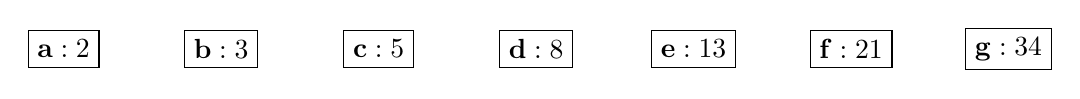
\begin{tikzpicture}[x=10mm, y=10mm]
	\node [rectangle, draw] (a) at (0,0) {$\mathbf{a}:2$};
	\node [rectangle, draw] (b) at (2,0) {$\mathbf{b}:3$};
	\node [rectangle, draw] (c) at (4,0) {$\mathbf{c}:5$};
	\node [rectangle, draw] (d) at (6,0) {$\mathbf{d}:8$};
	\node [rectangle, draw] (e) at (8,0) {$\mathbf{e}:13$};
	\node [rectangle, draw] (f) at (10,0) {$\mathbf{f}:21$};
	\node [rectangle, draw] (g) at (12,0) {$\mathbf{g}:34$};
\end{tikzpicture}

\vskip 36pt
$$Q = \{a:2, b:3, c:5, d:8, e:13, f:21, g:34\}$$

\begin{tikzpicture}[x=10mm, y=20mm]
	\node [rectangle, draw] (a) at (0,0) {$\mathbf{a}:2$};
	\node [rectangle, draw] (b) at (2,0) {$\mathbf{b}:3$};
	\node [rectangle, draw] (c) at (4,1) {$\mathbf{c}:5$};
	\node [rectangle, draw] (d) at (6,1) {$\mathbf{d}:8$};
	\node [rectangle, draw] (e) at (8,1) {$\mathbf{e}:13$};
	\node [rectangle, draw] (f) at (10,1) {$\mathbf{f}:21$};
	\node [rectangle, draw] (g) at (12,1) {$\mathbf{g}:34$};
	\node [ellipse, draw] (ab) at (1,1) {$\mathbf{ab}:5$};
	\foreach \from/\to in {a/ab}
		\draw (\from) -- (\to) node [midway, left] {0};
	\foreach \from/\to in {b/ab}
		\draw (\from) -- (\to) node [midway, right] {1};
\end{tikzpicture}


\vskip 36pt
$$Q = \{c:5, d:8, e:13, f:21, g:34, ab:5\}$$

\begin{tikzpicture}[x=10mm, y=20mm]
	\node [rectangle, draw] (a) at (0,0) {$\mathbf{a}:2$};
	\node [rectangle, draw] (b) at (2,0) {$\mathbf{b}:3$};
	\node [rectangle, draw] (c) at (-1,1) {$\mathbf{c}:5$};
	\node [rectangle, draw] (d) at (6,2) {$\mathbf{d}:8$};
	\node [rectangle, draw] (e) at (8,2) {$\mathbf{e}:13$};
	\node [rectangle, draw] (f) at (10,2) {$\mathbf{f}:21$};
	\node [rectangle, draw] (g) at (12,2) {$\mathbf{g}:34$};

	\node [ellipse, draw] (ab) at (1,1) {$\mathbf{ab}:5$};
	\node [ellipse, draw] (abc) at (0,2) {$\mathbf{abc}:10$};

	\foreach \from/\to in {a/ab, c/abc}
		\draw (\from) -- (\to) node [midway, left] {0};
	\foreach \from/\to in {b/ab, ab/abc}
		\draw (\from) -- (\to) node [midway, right] {1};
\end{tikzpicture}

$$Q = \{d:8, e:13, f:21, g:34, abc:10\}$$

\begin{tikzpicture}[x=10mm, y=20mm]
	\node [rectangle, draw] (a) at (0,0) {$\mathbf{a}:2$};
	\node [rectangle, draw] (b) at (2,0) {$\mathbf{b}:3$};
	\node [rectangle, draw] (c) at (-1,1) {$\mathbf{c}:5$};
	\node [rectangle, draw] (d) at (-2,2) {$\mathbf{d}:8$};
	\node [rectangle, draw] (e) at (4,3) {$\mathbf{e}:13$};
	\node [rectangle, draw] (f) at (6,3) {$\mathbf{f}:21$};
	\node [rectangle, draw] (g) at (8,3) {$\mathbf{g}:34$};

	\node [ellipse, draw] (ab) at (1,1) {$\mathbf{ab}:5$};
	\node [ellipse, draw] (abc) at (0,2) {$\mathbf{abc}:10$};
	\node [ellipse, draw] (abcd) at (-1,3) {$\mathbf{abcd}:18$};

	\foreach \from/\to in {a/ab, c/abc, d/abcd}
		\draw (\from) -- (\to) node [midway, left] {0};
	\foreach \from/\to in {b/ab, ab/abc, abc/abcd}
		\draw (\from) -- (\to) node [midway, right] {1};
\end{tikzpicture}

$$Q = \{e:13, f:21, g:34, abcd:18\}$$

\begin{tikzpicture}[x=12mm, y=20mm]
	\node [rectangle, draw] (a) at (0,0) {$\mathbf{a}:2$};
	\node [rectangle, draw] (b) at (2,0) {$\mathbf{b}:3$};
	\node [rectangle, draw] (c) at (-1,1) {$\mathbf{c}:5$};
	\node [rectangle, draw] (d) at (-2,2) {$\mathbf{d}:8$};
	\node [rectangle, draw] (e) at (-3,3) {$\mathbf{e}:13$};
	\node [rectangle, draw] (f) at (4,4) {$\mathbf{f}:21$};
	\node [rectangle, draw] (g) at (6,4) {$\mathbf{g}:34$};

	\node [ellipse, draw] (ab) at (1,1) {$\mathbf{ab}:5$};
	\node [ellipse, draw] (abc) at (0,2) {$\mathbf{abc}:10$};
	\node [ellipse, draw] (abcd) at (-1,3) {$\mathbf{abcd}:18$};
	\node [ellipse, draw] (abcde) at (-2,4) {$\mathbf{abcde}:31$};

	\foreach \from/\to in {a/ab, c/abc, d/abcd, e/abcde}
		\draw (\from) -- (\to) node [midway, ellipse, fill=white] {0};
	\foreach \from/\to in {b/ab, ab/abc, abc/abcd, abcd/abcde}
		\draw (\from) -- (\to) node [midway, ellipse, fill=white] {1};
\end{tikzpicture}

$$Q = \{f:21, g:34, abcde:31\}$$

\begin{tikzpicture}[x=12mm, y=20mm]
	\node [rectangle, draw] (a) at (0,0) {$\mathbf{a}:2$};
	\node [rectangle, draw] (b) at (2,0) {$\mathbf{b}:3$};
	\node [rectangle, draw] (c) at (-1,1) {$\mathbf{c}:5$};
	\node [rectangle, draw] (d) at (-2,2) {$\mathbf{d}:8$};
	\node [rectangle, draw] (e) at (-3,3) {$\mathbf{e}:13$};
	\node [rectangle, draw] (f) at (-4,4) {$\mathbf{f}:21$};
	\node [rectangle, draw] (g) at (2,5) {$\mathbf{g}:34$};

	\node [ellipse, draw] (ab) at (1,1) {$\mathbf{ab}:5$};
	\node [ellipse, draw] (abc) at (0,2) {$\mathbf{abc}:10$};
	\node [ellipse, draw] (abcd) at (-1,3) {$\mathbf{abcd}:18$};
	\node [ellipse, draw] (abcde) at (-2,4) {$\mathbf{abcde}:31$};
	\node [ellipse, draw] (abcdef) at (-3,5) {$\mathbf{abcdef}:52$};

	\foreach \from/\to in {a/ab, c/abc, d/abcd, e/abcde, f/abcdef}
		\draw (\from) -- (\to) node [midway, ellipse, fill=white] {0};
	\foreach \from/\to in {b/ab, ab/abc, abc/abcd, abcd/abcde, abcde/abcdef}
		\draw (\from) -- (\to) node [midway, ellipse, fill=white] {1};
\end{tikzpicture}

$$Q = \{g:34, abcdef:52\}$$

\begin{tikzpicture}[x=12mm, y=20mm]
	\node [rectangle, draw] (a) at (0,0) {$\mathbf{a}:2$};
	\node [rectangle, draw] (b) at (2,0) {$\mathbf{b}:3$};
	\node [rectangle, draw] (c) at (-1,1) {$\mathbf{c}:5$};
	\node [rectangle, draw] (d) at (-2,2) {$\mathbf{d}:8$};
	\node [rectangle, draw] (e) at (-3,3) {$\mathbf{e}:13$};
	\node [rectangle, draw] (f) at (-4,4) {$\mathbf{f}:21$};
	\node [rectangle, draw] (g) at (-5,5) {$\mathbf{g}:34$};

	\node [ellipse, draw] (ab) at (1,1) {$\mathbf{ab}:5$};
	\node [ellipse, draw] (abc) at (0,2) {$\mathbf{abc}:10$};
	\node [ellipse, draw] (abcd) at (-1,3) {$\mathbf{abcd}:18$};
	\node [ellipse, draw] (abcde) at (-2,4) {$\mathbf{abcde}:31$};
	\node [ellipse, draw] (abcdef) at (-3,5) {$\mathbf{abcdef}:52$};
	\node [ellipse, draw] (abcdefg) at (-4,6) {$\mathbf{abcdefg}:86$};

	\foreach \from/\to in {a/ab, c/abc, d/abcd, e/abcde, f/abcdef, g/abcdefg}
		\draw (\from) -- (\to) node [midway, ellipse, fill=white] {0};
	\foreach \from/\to in {b/ab, ab/abc, abc/abcd, abcd/abcde, abcde/abcdef, abcdef/abcdefg}
		\draw (\from) -- (\to) node [midway, ellipse, fill=white] {1};
\end{tikzpicture}

$$Q = \{abcdefg:86\}$$

Prefix Codes

\begin{tabular}{>{\bf}l>{\tt}l}
	a & 111110 \cr
	b & 111111 \cr
	c & 11110 \cr
	d & 1110 \cr
	e & 110 \cr
	f & 10 \cr
	g & 0 \cr
	
\end{tabular}


\subsubsection{Spring 2019 \#S3}
	% S19 S3
	Show your construction of an optimal Huffman code for the set of 10 frequencies:  
	
	{\bf a}:2 {\bf b}:6 {\bf c}:5 {\bf d}:8 {\bf e}:13 {\bf f}:34 {\bf g}:34 {\bf h}:15 {\bf i}:27 {\bf j}:9

\subsubsection{Solution} \

$Q_0 = \{
	\underline{\mathbf{a}: 2}, \ 
	\mathbf{b}: 6, \ 
	\underline{\mathbf{c}: 5}, \ 
	\mathbf{d}: 8, \ 
	\mathbf{e}: 13, \ 
	\mathbf{f}: 34, \ 
	\mathbf{g}: 34, \ 
	\mathbf{h}: 15, \ 
	\mathbf{i}: 27, \ 
	\mathbf{j}: 9
	\}
$


$Q_1 = \{
	\underline{\mathbf{b}: 6}, \ 
	\mathbf{d}: 8, \ 
	\mathbf{e}: 13, \ 
	\mathbf{f}: 34, \ 
	\mathbf{g}: 34, \ 
	\mathbf{h}: 15, \ 
	\mathbf{i}: 27, \ 
	\mathbf{j}: 9, \
	\underline{\mathbf{ac}: 7} 
	\}
$

$Q_2 = \{
	\underline{\mathbf{d}: 8}, \ 
	\mathbf{e}: 13, \ 
	\mathbf{f}: 34, \ 
	\mathbf{g}: 34, \ 
	\mathbf{h}: 15, \ 
	\mathbf{i}: 27, \ 
	\underline{\mathbf{j}: 9}, \
	\mathbf{bac}: 13 
	\}
$

$Q_3 = \{
	\underline{\mathbf{e}: 13}, \ 
	\mathbf{f}: 34, \ 
	\mathbf{g}: 34, \ 
	\mathbf{h}: 15, \ 
	\mathbf{i}: 27, \ 
	\underline{\mathbf{bac}: 13}, \  
	\mathbf{dj}: 17
	\}
$

$Q_4 = \{
	\mathbf{f}: 34, \ 
	\mathbf{g}: 34, \ 
	\underline{\mathbf{h}: 15}, \ 
	\mathbf{i}: 27, \ 
	\underline{\mathbf{dj}: 17}, \ 
	\mathbf{ebac}: 26  
	\}
$

$Q_5 = \{
	\mathbf{f}: 34, \ 
	\mathbf{g}: 34, \ 
	\underline{\mathbf{i}: 27}, \ 
	\underline{\mathbf{ebac}: 26}, \   
	\mathbf{hdj}: 32
	\}
$

$Q_6 = \{
	\underline{\mathbf{f}: 34}, \ 
	\mathbf{g}: 34, \ 
	\underline{\mathbf{hdj}: 32}, \ 
	\mathbf{ebaci}: 53   
	\}
$

$Q_7 = \{
	\underline{\mathbf{g}: 34}, \ 
	\underline{\mathbf{ebaci}: 53}, \   
	\mathbf{hdjf}: 66
	\}
$

$Q_8 = \{
	\underline{\mathbf{hdjf}: 66}, \ 
	\underline{\mathbf{gebaci}: 87}   
	\}
$

$Q_9 = \{
	\mathbf{hdjfgebaci}: 153   
	\}
$

\

\hfil\begin{tikzpicture}[x=12mm, y=20mm]
	\node [rectangle, draw] (a) at (3,-6) {$\mathbf{a}:2$};
	\node [rectangle, draw] (b) at (2,-5) {$\mathbf{b}:6$};
	\node [rectangle, draw] (c) at (5,-6) {$\mathbf{c}:5$};
	\node [rectangle, draw] (d) at (-3,-4) {$\mathbf{d}:8$};
	\node [rectangle, draw] (e) at (1,-4) {$\mathbf{e}:13$};
	\node [rectangle, draw] (f) at (-1,-2) {$\mathbf{f}:34$};
	\node [rectangle, draw] (g) at (1,-2) {$\mathbf{g}:34$};
	\node [rectangle, draw] (h) at (-4,-3) {$\mathbf{h}:15$};
	\node [rectangle, draw] (i) at (4,-3) {$\mathbf{i}:27$};
	\node [rectangle, draw] (j) at (-1,-4) {$\mathbf{j}:9$};

	\node [ellipse, draw] (ac) at (4,-5) {$\mathbf{ac}:7$};
	\node [ellipse, draw] (bac) at (3,-4) {$\mathbf{bac}:13$};
	\node [ellipse, draw] (dj) at (-2,-3) {$\mathbf{dj}:17$};
	\node [ellipse, draw] (ebac) at (2,-3) {$\mathbf{ebac}:26$};
	\node [ellipse, draw] (hdj) at (-3,-2) {$\mathbf{hdj}:32$};
	\node [ellipse, draw] (ebaci) at (3,-2) {$\mathbf{ebaci}:53$};
	\node [ellipse, draw] (hdjf) at (-2,-1) {$\mathbf{hdjf}:66$};
	\node [ellipse, draw] (gebaci) at (2,-1) {$\mathbf{gebaci}:87$};
	\node [ellipse, draw] (hdjfgebaci) at (0,0) {$\mathbf{hdjfgebaci}:153$};

	\foreach \from/\to in {hdjfgebaci/hdjf, hdjf/hdj, gebaci/g, hdj/h, ebaci/ebac, dj/d, ebac/e, bac/b, ac/a}
		\draw (\from) -- (\to) node [midway, ellipse, fill=white] {0};
	\foreach \from/\to in {hdjfgebaci/gebaci, hdjf/f, gebaci/ebaci, hdj/dj, ebaci/i, dj/j, ebac/bac, bac/ac, ac/c}
		\draw (\from) -- (\to) node [midway, ellipse, fill=white] {1};
\end{tikzpicture}

Prefix Codes

\begin{tabular}{>{\bf}l>{\tt}l}
	a & 110110 \cr
	b & 11010 \cr
	c & 110111 \cr
	d & 0010 \cr
	e & 1100 \cr
	f & 01 \cr
	g & 10 \cr
	h & 000 \cr
	i & 111 \cr
	j & 0011 \cr
\end{tabular}


\subsubsection{Fall 2018 \#S6}
	% F18 #S6
	Show your construction of an optimal Huffman code for the set of 7 frequencies:  
	
	$\mathbf{a}: 3, \mathbf{b}: 12, \mathbf{c}: 5, \mathbf{d}: 20, \mathbf{e}:16, \mathbf{f}: 34, \mathbf{g}:18$

